\documentclass[12pt, letterpaper]{article}

\usepackage{graphicx}
\usepackage{amsmath}

\title{Drop Pinch-off Experiment}
\author{Jay Shen}
\date{February 2025}

\begin{document}

\maketitle

\section{Introduction}

The fall of a droplet, though ordinary, is a surprisingly rich and complex phenomenon. In lieu of mathematical solutions to the myriad fluid physics at play, how might we draw conclusions about the forces that dominate this process?

In this experiment, we conducted an observational analysis of a fluid dropping from a nozzle. In particular, we examined the moment of pinch-off, and, by measuring droplet neck radii, obtained data suggesting specific scaling law dynamics. 

\section{Methods}

The main goal of this lab was to analyze the scaling of the thinnest parts of the droplet neck, especially in the moments leading up to dropoff. Our modeling hypothesis was that the thinnest radius of the neck, $r$, should be related to the time till dropoff, $t_d - t$, by a power law: 
\[
    r = A(t_d - t)^\gamma
\]
Moving to log-scale admits:
\[
    \ln r = \gamma \ln (t_d - t) + \ln A
\]
Given measurements of $r$ and $t_d - t$, we can easily obtain estimates for $\gamma$ and $A$ by fitting a linear model to our data in log-scale. Furthermore, since we are mainly interested in $\gamma$, we do not need to worry about units, as any scalars factor out and do not affect the estimate of $\gamma$:
\begin{align*}
    \ln Br &= \gamma \ln (C(t_d - t)) + \ln A \\
    \ln r + \ln B &= \gamma \ln (t_d - t) + \gamma \ln C + \ln A \\
    \ln r &= \gamma \ln (t_d - t) + \text{Constant}
\end{align*}

To obtain our measurements, we filmed the fall of droplets using a high frame rate camera. Then, from the videos obtained, we took measurements of droplet features using the ImageJ software. In the experiments described in this report, measurements were taken by using a line measurement tool to draw a vertical line across the entire width of some feature. Then, we record the pixel length of the line and process it accordingly. Figure \ref{fig:measurement3} shows this workflow. 

\begin{figure}[!h]
    \centering
    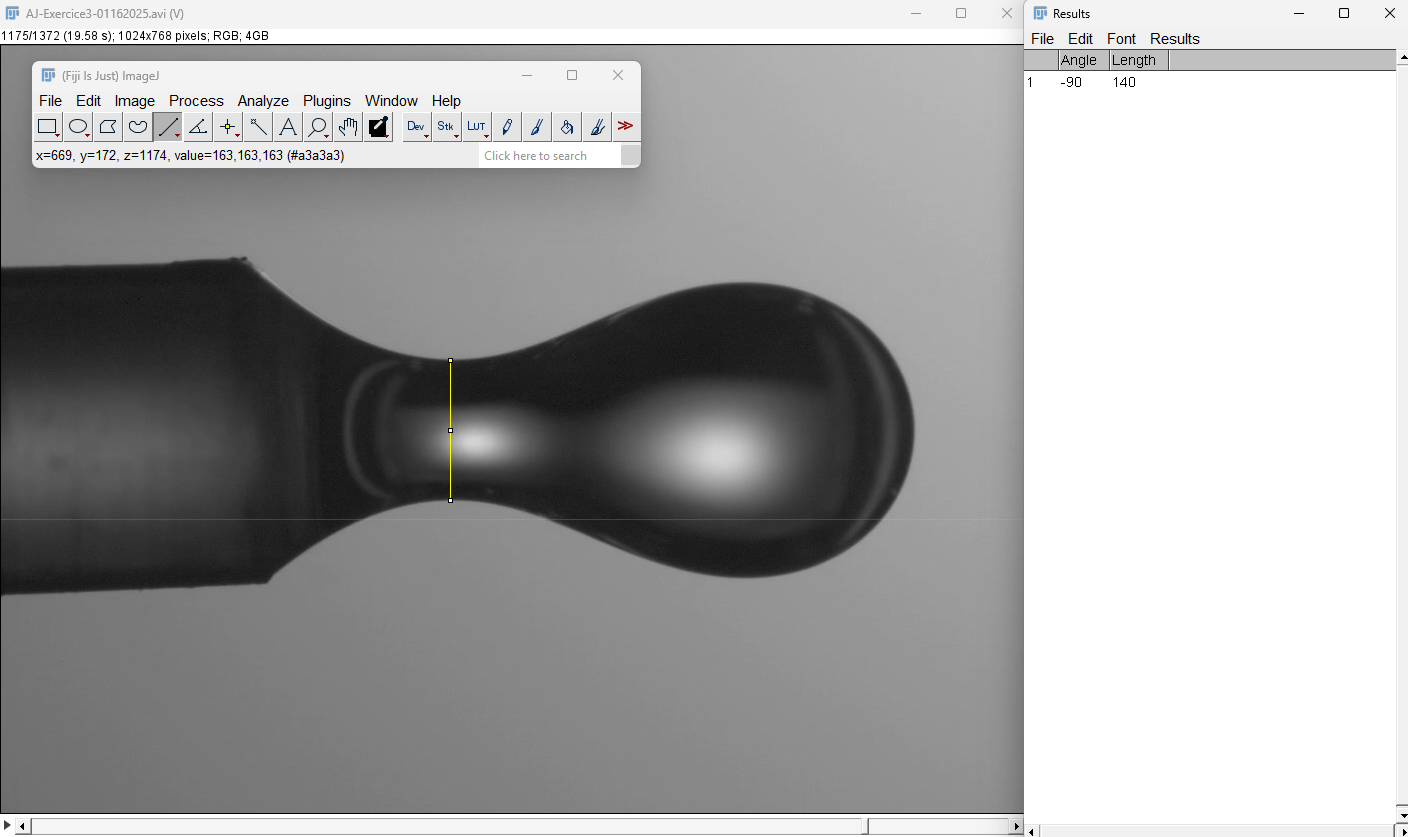
\includegraphics[width=0.75\textwidth]{experiment3/figures/screenshots/measurement3.png}
    \caption{A screenshot of the software we used for feature measurement. In the middle is a frame from the video of the droplet. We drew the yellow line to capture the diameter of the droplet neck. ImageJ reports the pixel length of this line on the right. }
    \label{fig:measurement3}
\end{figure}

The uncertainties in our length measurements were determined by the pixelation of the videos. Looking at the fuzziness of the image, we hand estimated a rough uncertainty in pixels for each measurement. For example, Figure \ref{fig:measurement2-zoom} shows a width measurement of a droplet feature. The uncertainty here was determined to be $6$ pixels given an $\sim 3$ pixel ambiguity on each side. 

\begin{figure}[!h]
    \centering
    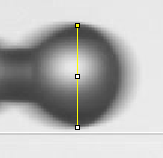
\includegraphics[width=0.75\textwidth]{experiment3/figures/screenshots/measurement2-zoom.png}
    \caption{A measurement taken of a fuzzy frame. }
    \label{fig:measurement2-zoom}
\end{figure}

We also reported the uncertainty in our timestamps, which are discretized to the frame rate. The error, when considering this discrete sampling, is conservatively $\frac{1}{2f}$ for frame rate $f$. 

From these measurement uncertainties, margins of error can be derived for all fitted quantities via covariances. We leave this computation to our fitting software of choice. 

\section{Results}

\subsection{Viscosity}

Jiang et al. \cite{jiang} report that low viscosity liquids exhibit an exponent of $\gamma = \frac{2}{3}$ throughout the pinch-off process. To test this result, we took measurements around the bottom pinch-off of tap water droplets. Water has a low viscosity on the order of $1$ cP. 

\begin{figure}[!h]
    \centering
    \includegraphics[width=0.75\textwidth]{}
    \caption{Pinch-off measurements for water}
    \label{fig:water1}
\end{figure}

Figure \ref{fig:water1} shows our measurements in log-scale. The plot appears generally linear, so we go ahead and fit our power law model. 

\begin{figure}[!h]
    \centering
    \includegraphics[width=0.75\textwidth]{}
    \caption{Fit of measurements for water droplet.}
    \label{fig:water-fit1}
\end{figure}

The fitted curve is shown in Figure \ref{fig:water-fit1}. The expected exponent $\gamma = \frac{2}{3}$ falls just outside our fitted exponent's margin of error $\gamma = $. However, it is close enough that the discrepancy could plausibly be a result of mishandling of uncertainty, impurities within the water we use, or biases within our measurement procedure. We also note the ambiguous oscillatory behavior of residuals in the early stage. The nature of this should be explored in future work. 

To elucidate these results, we conducted a second round of measurements, this time focusing on the moments just before pinch-off. Our measurements and a fit are shown in Figure \ref{fig:water-fit2}

\begin{figure}[!h]
    \centering
    \includegraphics[width=0.75\textwidth]{}
    \caption{Fit of measurements for water droplet.}
    \label{fig:water-fit2}
\end{figure}

Though our uncertainties here were high due to the poor quality of our video, the expected value of $\gamma = \frac{2}{3}$ does fall within our margin of error $\gamma = $. Though these results do not offer the definitive evidence we hoped to find, they continue to affirm the general ballpark of exponents we hoped to confirm. 

Jiang et al. also report that for high viscosity liquids, the early stage of the drop-off exhibits exponent of $\gamma = \frac{2}{3}$ as in the low viscosity case. However, in the late stages, the exponent should change to $\gamma = 1$. These two exponents correspond to inertial and viscous regimes, respectively. We explored this claim by taking measurements of the bottom pinch-off of a $20/40$ mixture of water and glycerine. Glycerine is highly viscous, measuring on the order of $870,000$ cP. 

\begin{figure}[!h]
    \centering
    \includegraphics[width=0.75\textwidth]{}
    \caption{Pinch-off measurements for 20/40 glycerine mixture}
    \label{fig:glycerine}
\end{figure}

Figure \ref{fig:glycerine} shows our collected data again plotted in log-scale. Unlike water, we observe a slight non-linearity $0.00079$ seconds before pinch-off. Elsewhere, however, the plot is generally linear. With this in mind, we fit two separate power laws to the two regions on either side of the non-linearity. 

\begin{figure}[!h]
    \centering
    \includegraphics[width=0.75\textwidth]{}
    \caption{Fit for early stage of 20/40 glycerine mixture droplet.}
    \label{fig:glycerine-fit1}
\end{figure}

\begin{figure}[!h]
    \centering
    \includegraphics[width=0.75\textwidth]{}
    \caption{Fit for later stage of 20/40 glycerine mixture droplet.}
    \label{fig:glycerine-fit2}
\end{figure}

Figures \ref{fig:glycerine-fit1} and \ref{fig:glycerine-fit2} show curves fitted to the early and later stages of the pinch-off, respectively. Our expected exponents of $\gamma = \frac{2}{3}$ and $\gamma = 1$ fall within our fit margins of error for both regions. This offers strong evidence in support of Jiang et al. claims. We report our fitted exponents in Table \ref{tab:exponents}

\begin{table}[!h]
    \centering
    \begin{tabular}{|c|c|c|}
        \hline
         & $\gamma$ & Domain \\
        \hline
        Water & $0.61 \pm 0.03$ & $0.00011 < t_d - t < 0.0043$ \\
        \hline
        Glycerine Mix & $0.90 \pm 0.26$ & $0.00011 < t_d - t < 0.00091$ \\
        & $0.72 \pm 0.07$ & $0.0010 < t_d - t < 0.0032$ \\
        \hline
    \end{tabular}
    \caption{Fitted scaling exponents for water and glycerine mix. }
    \label{tab:exponents}
\end{table}

\subsection{Symmetry}

Thus far, we have examined the pinch-off of the droplets at the bottom of the neck. But what about the pinch-off of the neck from the nozzle? Ostensibly, the physics should be same and we ought to extract the same power laws. 

To test this hypothesis, we performed the same procedure except this time focusing on the top pinch-off. Our collected measurements, along with a power-law fit, are shown in Figure \ref{fig:top-pinchoff}

\begin{figure}[!h]
    \centering
    \includegraphics[width=0.75\textwidth]{}
    \caption{Pinch-off measurements and fit for top pinch-off}
    \label{fig:top-pinchoff}
\end{figure}

We observe an exponent of $\gamma=0.64 \pm 0.04$, which contains the expected value $\gamma=\frac{2}{3}$ within the reported margin of error. This offers strong evidence in support of our hypothesis that scaling laws do not change whether we examine the top or bottom pinch-off. 

\subsection{Repeatability}

We also ask to what degree our measurements for one droplet reflect generic phenomena that may be observed across all drops. That is, are these experiments repeatable? Or are there large, systematic differences between successive drops that we must account for? 

In this section, we conduct a preliminary investigation into repeatability by measuring the maximum width of the droplet neck. Using a similar setup as before, we take high-frame rate videos of the droplet neck after complete pinch-off, and then take measurements each frame using software. Our quantification of uncertainty follows the same heuristic described above. Figure \ref{fig:measurment2} shows an example of our workflow. 
\begin{figure}[!h]
    \centering
    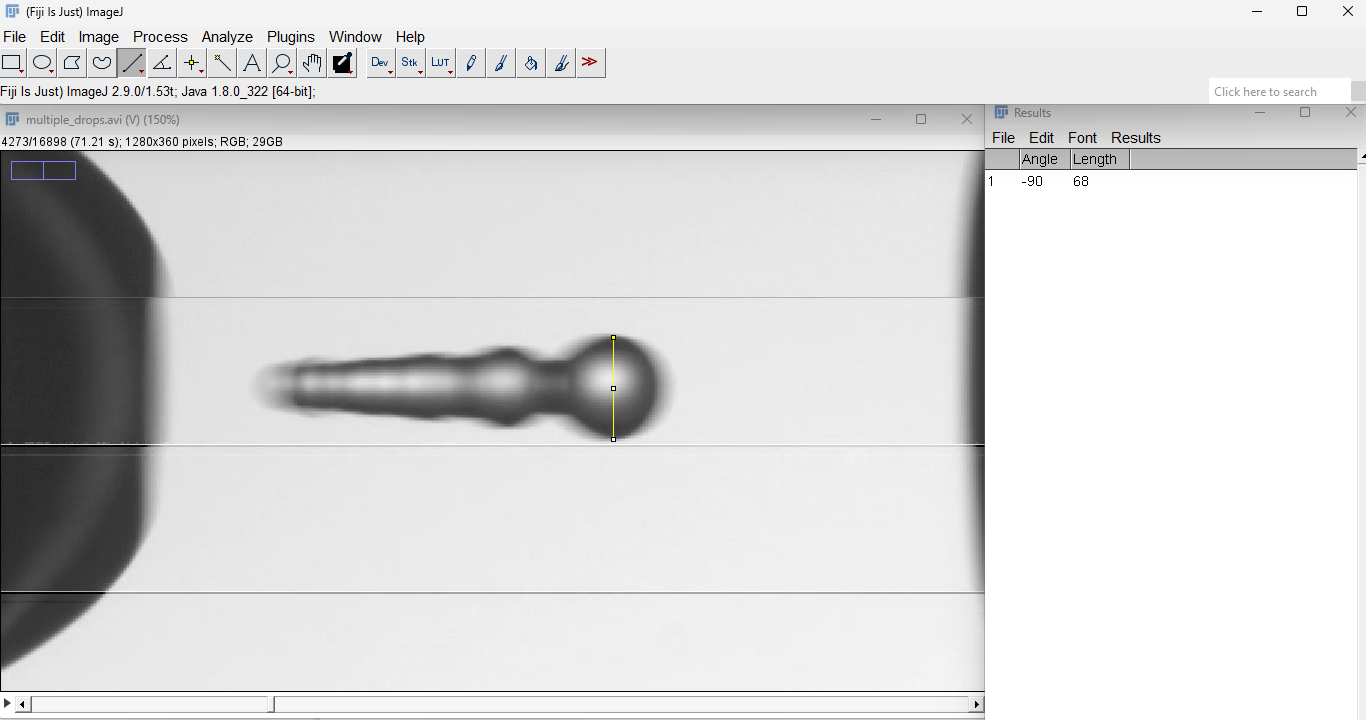
\includegraphics[width=0.75\textwidth]{experiment3/figures/screenshots/measurement2.png}
    \caption{Screenshot of our setup for measuring neck max width. }
    \label{fig:measurement2}
\end{figure}

\begin{figure}[!h]
    \centering
    \includegraphics[width=0.75\textwidth]{experiment3/figures/}
    \caption{Neck max-width measurements from 4 successive water droplets plotted together. }
    \label{fig:repeatability1}
\end{figure}

Our neck max-width measurements are plotted in Figure \ref{fig:repeatability1}. Evidently, the maximum width of the neck evolves similarly across all measured drops, increasing rapidly after drop-off before peaking and then falling off. 
\begin{figure}[!h]
    \centering
    \includegraphics[width=0.75\textwidth]{experiment3/figures/}
    \caption{Mean neck maximum width measurements with included uncertainty margins. }
    \label{fig:repeatability-mean}
\end{figure}
Figure \ref{fig:repeatability-mean} summarizes this relationship by plotting the mean and standard deviation bounds of the measurements at each time step. Now, the sample size is small, but the uncertainties observed are fairly low, and the general shape of the curve we observe likely holds in general. However, we followed up by investigating possible time-dependencies in the behavior of successive drops. Figure \ref{eq:equation1} shows the residuals of each drop from the mean curve. 

\begin{figure}[!h]
    \centering
    \includegraphics[width=0.75\textwidth]{experiment3/figures/}
    \caption{Residuals of neck max-width measurements. There is visual evidence of homoskedasticity. }
    \label{fig:repeatability1}
\end{figure}

From this plot, we conclude that the series is likely homoscedastic, as the residuals seem random and independent of time and drop index. This conclusion affirms our hypothesis that the drop experiments we have conducted thus far are repeatable. More data and the application of regression analysis tests will be useful in clarifying the repeatability of drop pinch-off. 

\section{Conclusion}

In this lab, we observed the extent to which power laws are good models for droplet features. Using a fairly straightforward setup, we took rough measurements which our model was then fit to. We confirmed our model hypothesis, and also estimated exponents that mostly agreed with those reported in literature. Finally, we conducted a quick verification of the experiment's repeatability, and found evidence in its favor. 

In the future, it would be wise to collect more thorough and ample data to reevaluate our results with greater statistical power. 

\begin{thebibliography}{!h}
    \bibitem{jiang}
    Xiaofeng Jiang, Enle Xu, Xianliang Meng, Huai Z. Li, The effect of viscosity ratio on drop pinch-off dynamics in two-fluid flow, Journal of Industrial and Engineering Chemistry, Volume 91, 2020, Pages 347-354, ISSN 1226-086X, https://doi.org/10.1016/j.jiec.2020.08.019.
\end{thebibliography}

\end{document}
